%%%%%%%%%%%%%%%%%%%%%%%%%%%%%%%%%%%%%%%%%
% Jacobs Landscape Poster
% LaTeX Template
% Version 1.1 (14/06/14)
%
% Created by:
% Computational Physics and Biophysics Group, Jacobs University
% https://teamwork.jacobs-university.de:8443/confluence/display/CoPandBiG/LaTeX+Poster
% 
% Further modified by:
% Nathaniel Johnston (nathaniel@njohnston.ca)
%
% This template has been downloaded from:
% http://www.LaTeXTemplates.com
%
% License:
% CC BY-NC-SA 3.0 (http://creativecommons.org/licenses/by-nc-sa/3.0/)
%
%%%%%%%%%%%%%%%%%%%%%%%%%%%%%%%%%%%%%%%%%

%----------------------------------------------------------------------------------------
%	PACKAGES AND OTHER DOCUMENT CONFIGURATIONS
%----------------------------------------------------------------------------------------

\documentclass[final, 20pt]{beamer}
\usepackage{array}
\newcolumntype{M}[1]{>{\centering\arraybackslash}m{#1}}
\usepackage{xcolor,colortbl}
\usepackage[size=a0,scale=1.45]{beamerposter} % Use the beamerposter package for laying out the poster
\usepackage{hyperref}
\renewcommand{\baselinestretch}{1.1} 
\usepackage{tikz}
%\usetikzlibrary{matrix}
%\tikzset{%
%  highlight/.style={rectangle,fill=blue,draw=none,fill opacity=.1,inner sep=0pt}
%}
%\definecolor{cardinalred}{RGB}{177, 4, 14}
\definecolor{cardinalred}{RGB}{140, 21, 21}

\usetheme{confposter} % Use the confposter theme supplied with this template

\setbeamercolor{block title}{fg=cardinalred,bg=white} % Colors of the block titles
\setbeamercolor{block body}{fg=black,bg=white} % Colors of the body of blocks
\setbeamercolor{block alerted title}{fg=white,bg=cardinalred} % Colors of the highlighted block titles
\setbeamercolor{block alerted body}{fg=black,bg=sandstone} % Colors of the body of highlighted blocks
% Many more colors are available for use in beamerthemeconfposter.sty

%-----------------------------------------------------------
% Define the column widths and overall poster size
% To set effective sepwid, onecolwid and twocolwid values, first choose how many columns you want and how much separation you want between columns
% In this template, the separation width chosen is 0.024 of the paper width and a 4-column layout
% onecolwid should therefore be (1-(# of columns+1)*sepwid)/# of columns e.g. (1-(4+1)*0.024)/4 = 0.22
% Set twocolwid to be (2*onecolwid)+sepwid = 0.464
% Set threecolwid to be (3*onecolwid)+2*sepwid = 0.708

\newlength{\sepwid}
\newlength{\onecolwid}
\newlength{\twocolwid}
\newlength{\threecolwid}
\setlength{\paperwidth}{54in} % A0 width: 46.8in
\setlength{\paperheight}{36in} % A0 height: 33.1in
\setlength{\sepwid}{0.024\paperwidth} % Separation width (white space) between columns
\setlength{\onecolwid}{0.22\paperwidth} % Width of one column
\setlength{\twocolwid}{0.464\paperwidth} % Width of two columns
\setlength{\threecolwid}{0.708\paperwidth} % Width of three columns
\setlength{\topmargin}{-0.5in} % Reduce the top margin size
%-----------------------------------------------------------
\usepackage{graphicx}  % Required for including images
\usepackage{booktabs} % Top and bottom rules for tables


\addtobeamertemplate{headline}{} 
{
\begin{tikzpicture}[remember picture,overlay] 
\node [shift={(10 cm,-6cm)}] at (current page.north west) {
\includegraphics[height=10cm]{Stanford-Logo.png}}; 
\end{tikzpicture} 
}
%----------------------------------------------------------------------------------------
%	TITLE SECTION 
%----------------------------------------------------------------------------------------
\title{Randomized Iterative Algorithms for Solving Elliptic PDEs} % Poster title

\author{Jialun Zhang\textsuperscript{1}}
\institute{[1] ICME, Stanford University} 



%----------------------------------------------------------------------------------------

\begin{document}

\addtobeamertemplate{block end}{}{\vspace*{2ex}} % White space under blocks
\addtobeamertemplate{block alerted end}{}{\vspace*{2ex}} % White space under highlighted (alert) blocks

\setlength{\belowcaptionskip}{2ex} % White space under figures
\setlength\belowdisplayshortskip{2ex} % White space under equations

\begin{frame}[t] % The whole poster is enclosed in one beamer frame

\begin{columns}[t] % The whole poster consists of three major columns, the second of which is split into two columns twice - the [t] option aligns each column's content to the top

\begin{column}{\sepwid}\end{column} % Empty spacer column

\begin{column}{\onecolwid} % The first column

\begin{alertblock}{Abstract}
\begin{flushleft}
We consider the classical problem of solving an elliptic partial differential equation on a circular disk in $\mathbb{R}^2$. These equations can be solved by various deterministic algorithms such as finite differences and finite elements. The finite element method in particular projects the equation onto a finite-dimensional subspace by discretizing the domain and considering piece-wise linear functions. This usually gives us a linear system of the form $Au=b$, where $A$ is a large sparse matrix that is positive semi-definite. For these kind of linear systems, iterative algorithms such as the conjugate gradient method has been widely used. In this poster, we chiefly consider two \textit{randomized} iterative methods, namely the \textbf{randomize coordinate descent} method and \textbf{Gaussian sampling}. 
\end{flushleft}
\end{alertblock}

\begin{alertblock}{Iterative Randomized Least Squares}
\begin{flushleft}

Many randomized iterative algorithms can be described as a specific case of the following algorithm: for some positive definite $B\in\mathbb{R}^{n\times n}$ and random matrix $S\in\mathbb{R}^{m\times q}$, choose an initial $x^{(0)}$ and apply updates of the form
\begin{align*}
	x^{k+1}=\arg \min _{x \in \mathbb{R}^{n}}\left\|x-x^{k}\right\|_{B}^{2} \quad \text {subject to} \quad S^{T} A x=S^{T} b,
\end{align*}
where $\|x\|_B = \sqrt{x^TBx}$. Analytically, this can be written as
\begin{align*}
	x^{k+1}=x^{k}-B^{-1} A^{T} S\left(S^{T} A B^{-1} A^{T} S\right)^{\dagger} S^{T}\left(A x^{k}-b\right).\label{algebra_update}
\end{align*}

\end{flushleft}
\end{alertblock}
\end{column} 

\begin{column}{\sepwid}\end{column} % Empty spacer column

\begin{column}{\onecolwid}


\begin{block}{Randomized Coordinate Descent}
\begin{flushleft}
Assume that $A$ is positive definite, so we can choose $B=A$ and $S=e^i$. This yields the following update
\begin{align}
x^{k+1}=x^{k}-\frac{\left(A_{i :}\right)^{T} x^{k}-b_{i}}{A_{i i}} e^{i}.
\end{align}
The convergence can be written as
\begin{align}
\mathbf{E}\left[\left\|x^{k}-x^{*}\right\|_{A}^{2}\right] \leq\left(1-\frac{\lambda_{\min }(A)}{\operatorname{Tr}(A)}\right)^{k}\left\|x^{0}-x^{*}\right\|_{A}^{2}.
\end{align}
The algorithm has an iteration complexity of
\[
O\left(\operatorname{Tr}(A) / \lambda_{\min }(A)\right),
\]
while CG has an iteration complexity of $$O(\sqrt{\lambda_{\max }(A) / \lambda_{\min }(A)}).$$ The advantage is that each iteration costs $O(n)$ instead of $O(n^2)$. 
\end{flushleft}
\end{block}
\begin{block}{Gaussian Sampling}
\begin{flushleft}
Assume that $A$ is positive definite, so we can choose $B=A$. Let $S = \zeta \sim N(0, \Sigma)$. This yields the update 
\begin{align}
x^{k+1}=x^{k}-\frac{\eta^{T}\left(A x^{k}-b\right)}{\|\eta\|_{A}^{2}} \eta.
\end{align}
The convergence can be written as
\begin{align}
\mathbf{E}\left[\left\|x^{k}-x^{*}\right\|_{A}^{2}\right] \leq\rho^k \left\|x^{0}-x^{*}\right\|_{A}^{2},
\end{align}
where 
\begin{align}
1-\frac{1}{n} \leq \rho \leq 1-\frac{2}{\pi} \frac{\lambda_{\min }(\Omega)}{\operatorname{Tr}(\Omega)},
\end{align}
where $\Omega \stackrel{\mathrm{def}}{=} B^{-1 / 2} A^{\top} \Sigma A B^{-1 / 2}$.
\end{flushleft}
\end{block}



%----------------------------------------------------------------------------------------

\end{column}
\begin{column}{\sepwid}\end{column} 
\begin{column}{\onecolwid} 
%----------------------------------------------------------------------------------------
%----------------------------------------------------------------------------------------
\begin{block}{Elliptic PDEs and Finite Elements}
\begin{flushleft}
We consider a partial differential equation of the form
\[
\mathcal{A} u :=-\nabla \cdot(a \nabla u)=f \quad \text { in } \Omega, \quad \text { with } u=0 \quad \text { on } \Gamma.
\]
We discretize domain as shown in Figure 1.
\begin{figure*}
	\centering
	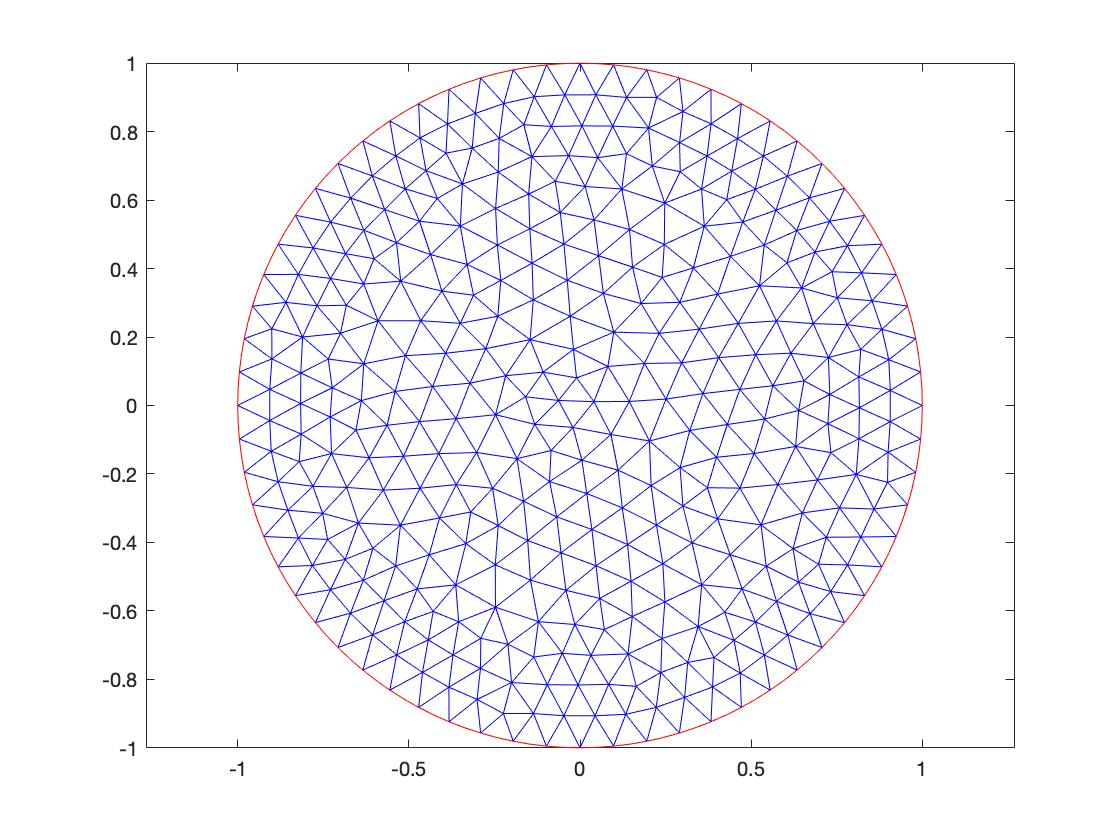
\includegraphics[scale=0.8]{mesh}
\end{figure*}

By considering piecewise linear functions defined on the triangles, we attain an equation of the form $Au=b$, where $A$ is sparse and SPD.
\end{flushleft}

%----------------------------------------
\end{block}

\begin{block}{Convergence}
Convergence for Randomized Coordinate Descent. 
\begin{flushleft}
\begin{figure*}
	\centering
	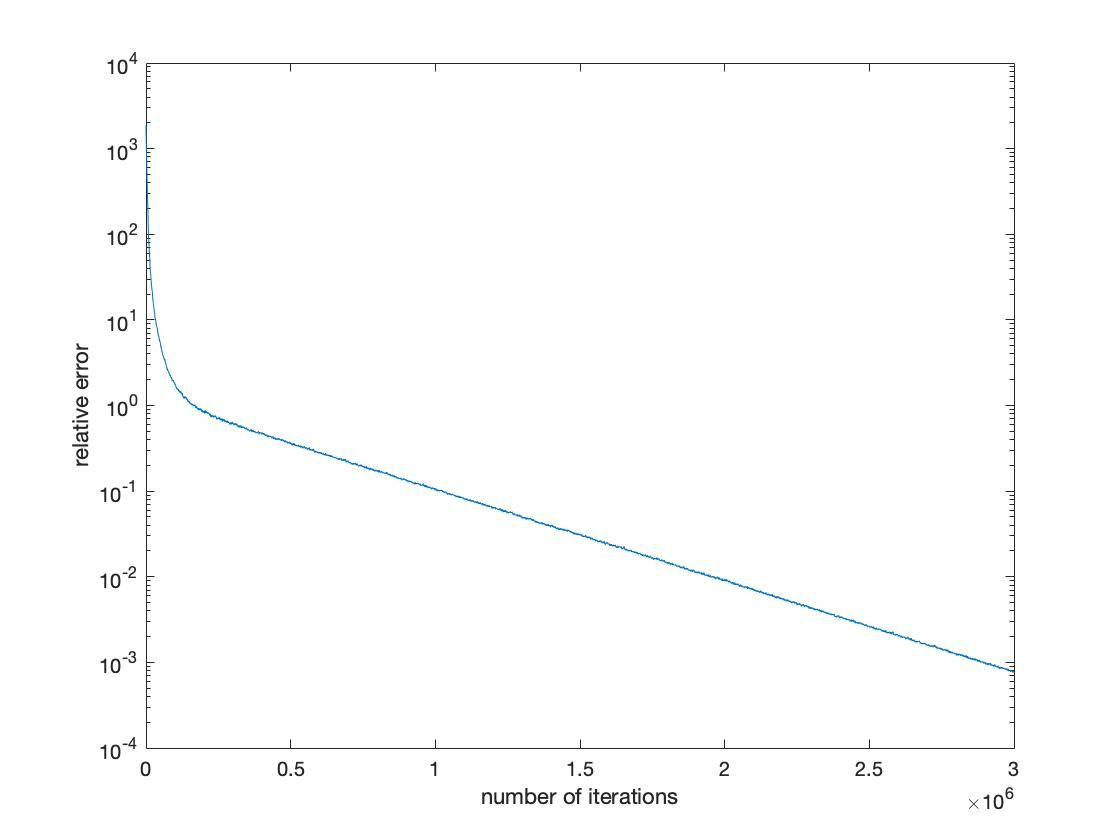
\includegraphics[scale=0.7]{cd_pd_convergence}
\end{figure*}
\end{flushleft}

%----------------------------------------
\end{block}



%----------------------------------------------------------------------------------------
\end{column}
\begin{column}{\sepwid}\end{column} % Empty spacer column

\begin{column}{\onecolwid} % The third column

%----------------------------------------------------------------------------------------
%	CONCLUSION
\begin{block}{Convergence (continued)}
\begin{flushleft}
Convergence for Gaussian Sampling. 
\begin{figure*}
	\centering
	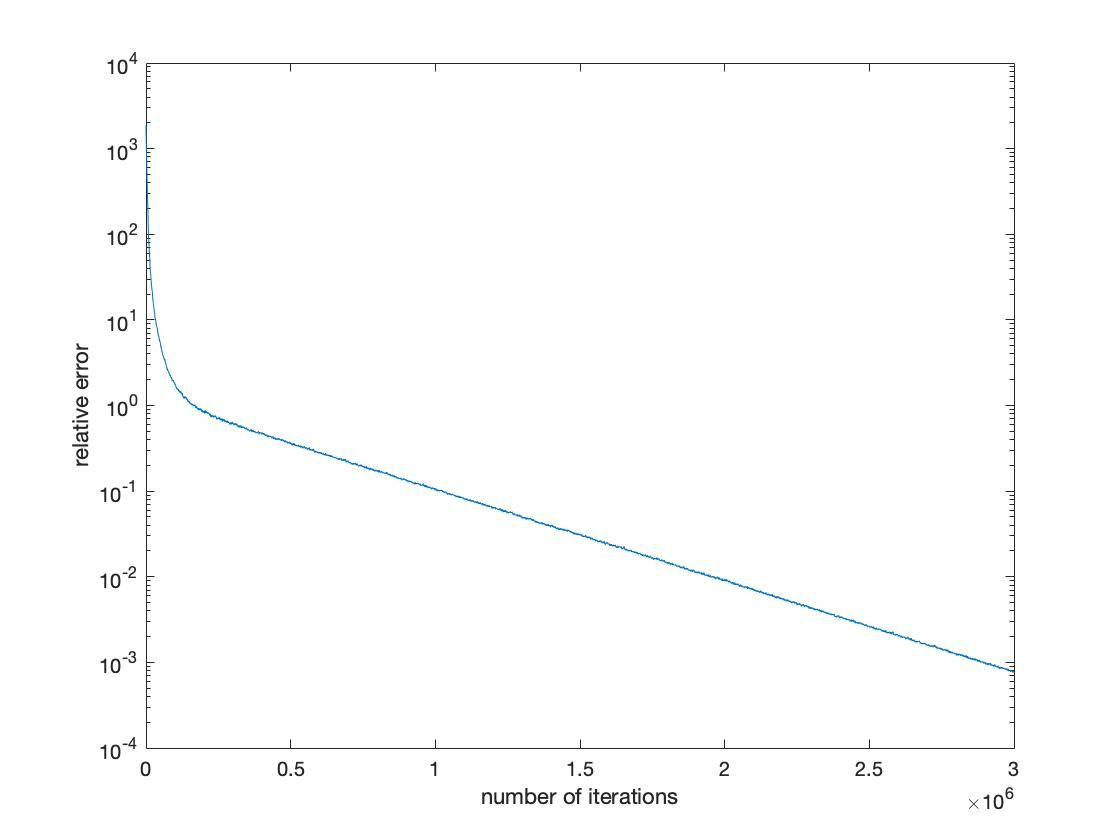
\includegraphics[scale=0.7]{cd_pd_convergence}
\end{figure*}
\end{flushleft}
\end{block}

\begin{alertblock}{Discussion}
\begin{flushleft}
Due to limitations in computation, we chose a mesh size of $h=0.1$ which results in a SPD matrix of size $O(10^3)$. On these scales, the randomized methods perform much slower compared to CG. The number of iterations it takes to converge is almost squared. However, it is clear that these methods do eventually converge to the optimal solution, and can be useful when $A$ is sufficiently large. 
\end{flushleft}
\end{alertblock}

%----------------------------------------------------------------------------------------
%	REFERENCES
%----------------------------------------------------------------------------------------

\begin{alertblock}{Reference}
[1] Gower, Robert M. "Sketch and project: randomized iterative methods for linear systems and inverting matrices." arXiv preprint arXiv:1612.06013 (2016).

[2] Larsson, Stig, and Vidar Thomée. Partial differential equations with numerical methods. Vol. 45. Springer Science & Business Media, 2008.

\noident
\vspace{0.5cm}

\vspace{0.5cm}

\end{alertblock}

%----------------------------------------------------------------------------------------
%	ACKNOWLEDGEMENTS
%----------------------------------------------------------------------------------------
%
%\setbeamercolor{block title}{fg=red,bg=white} % Change the block title color
%
%\begin{block}{Acknowledgements}
%
%\small{\rmfamily{Nam mollis tristique neque eu luctus. Suspendisse rutrum congue nisi sed convallis. Aenean id neque dolor. Pellentesque habitant morbi tristique senectus et netus et malesuada fames ac turpis egestas.}} \\
%
%\end{block}

%----------------------------------------------------------------------------------------
%	CONTACT INFORMATION
%----------------------------------------------------------------------------------------

%\setbeamercolor{block alerted title}{fg=black,bg=norange} % Change the alert block title colors
%\setbeamercolor{block alerted body}{fg=black,bg=white} % Change the alert block body colors
%
%\begin{alertblock}{Contact Information}
%
%\begin{itemize}
%\item Web: \href{http://www.university.edu/smithlab}{http://www.university.edu/smithlab}
%\item Email: \href{mailto:john@smith.com}{john@smith.com}
%\item Phone: +1 (000) 111 1111
%\end{itemize}
%
%\end{alertblock}


%----------------------------------------------------------------------------------------

\end{column} % End of the third column

\end{columns} % End of all the columns in the poster

\end{frame} % End of the enclosing frame

\end{document}
